\begin{annexesenv}

% Imprime uma página indicando o início dos anexos
\partannexes

\chapter{INA326 complete Schematic.}

\begin{figure}[!htpb]
  \centering
  \caption{INA326 Complete Schematic}
  \label{INA-complete-schematic}
  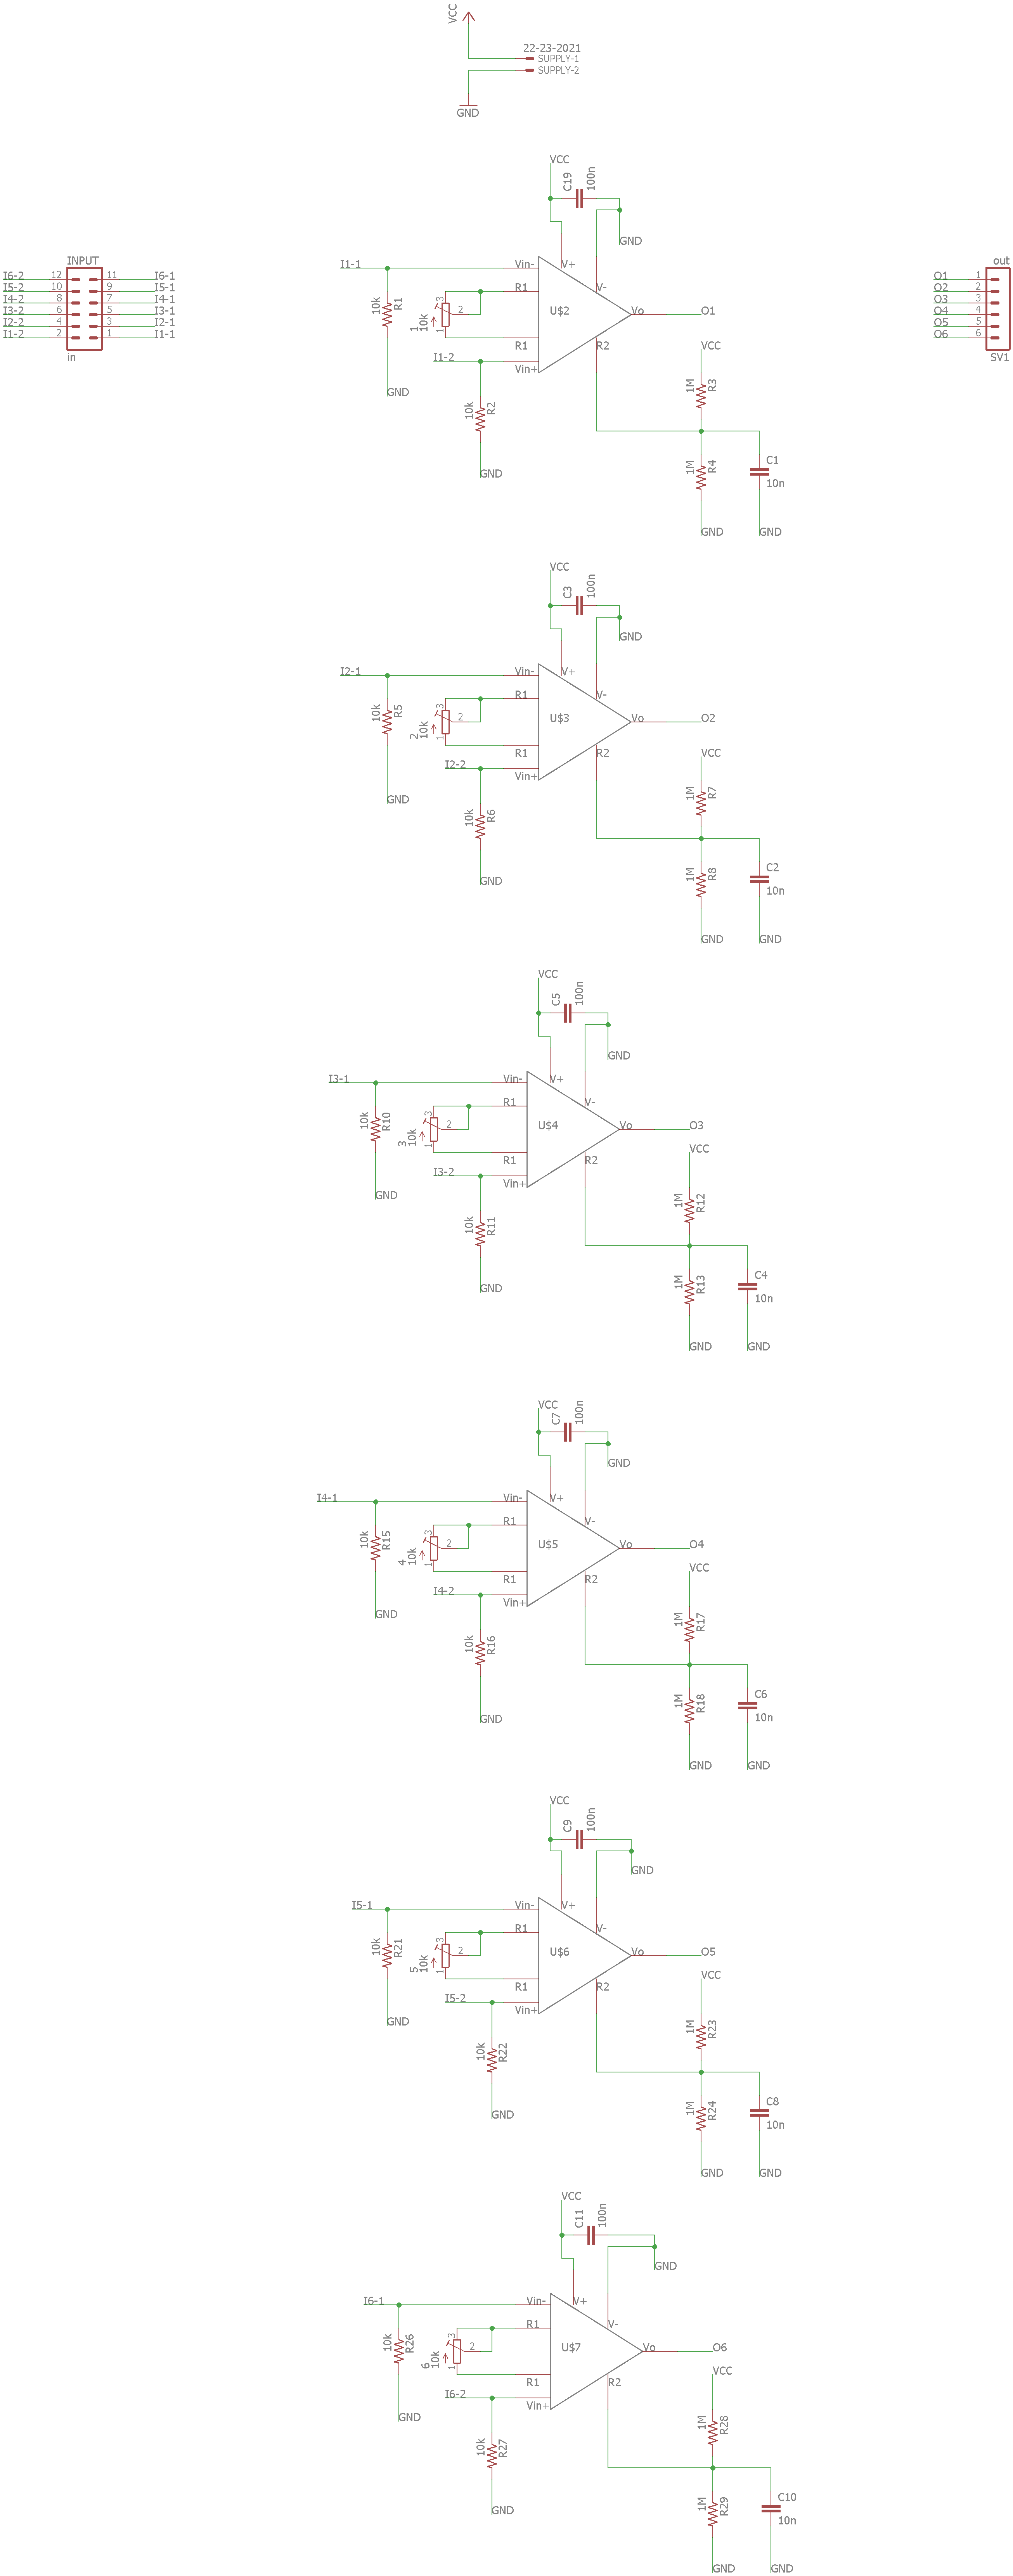
\includegraphics[scale=0.35]{images/INA/complete-schematic}
  \legend{Source: authors}
\end{figure}

\chapter{Prototype Cost Table.}

Costs are given on United States Dolar.\\
\begin{table}[htb]
  \begin{center}
    \ABNTEXreducedfont
    \caption[Prototype Board Cost Table]{Prototype Board Cost Table}
    \label{Prototype-cost}
    \begin{tabular}{c|c|c}
      \textbf{Component} & \textbf{Quantity} & \textbf{Cost} \\
    \hline
    \hline
    INA326 & 6 & 37.38\\ \hline
    10k$\Omega$ Trimmer Potentiometer & 6 & 7.50 \\ \hline
    10nF Ceramic Capacitor & 6 & 2.34 \\ \hline
    100nF Electrolytic Capacitor & 6 & 0.47 \\ \hline
    10k$\Omega$ Resistor 5$\%$ tolerance & 12 & 0.62 \\ \hline
    1M$\Omega$ Resistor 5$\%$ tolerance & 12 & 0.62 \\ \hline
    Pin bar 1x40 & 1 & 0.93 \\ \hline
    PCB & 2 & 15.57 \\ \hline
    Pickup Base and Cover & 1 & 4.68 \\ \hline
    Magnets & 6 & 9.37 \\ \hline
    Copper wire & 0.2969oz & 0.18 \\ \hline
  \end{tabular}
  \legend{Source: authors}
\end{center}
\end{table}

Total production cost for the prototype - 79.66

\chapter{Production Cost Table.}

Costs are given on United States Dollar for production of 1000 devices.\\
\begin{table}[htb]
  \begin{center}
    \ABNTEXreducedfont
    \caption[Production Board Prediction Cost Table]{Production Board Prediction Cost Table}
    \label{Production-cost}
    \begin{tabular}{c|c|c|c}
      \textbf{Component} & \textbf{Quantity} & \textbf{Cost per Component} & \textbf{Total Cost} \\
     \hline
     \hline
    INA326 & 6 & 2.53071 & 15.18\\ \hline
    10k$\Omega$ SMD Trimmer Potentiometer & 6 & 2.16050 & 12.96 \\ \hline
    10nF SMD Ceramic Capacitor & 6 & 0.00233 & 0.01 \\ \hline
    100nF Electrolytic Capacitor & 6 & 0.04431 & 0.27 \\ \hline
    10k$\Omega$ SMD Resistor 1$\%$ tolerance & 12 & 0.00649 & 0.08 \\ \hline
    1M$\Omega$ SMD Resistor 1$\%$ tolerance & 12 & 0.00671 & 0.08 \\ \hline
    Pin bar 1x40 & 1 & 0.62240 & 0.62 \\ \hline
    PCB & 1 & 0.22 & 0.22 \\ \hline
    Pickup Base and Cover & 1 & 4.68 & 4.68 \\ \hline
    Magnets & 6 & 0.82 & 4.92  \\ \hline
    Copper wire & 0.5938oz & 2.01/oz & 1.19  \\ \hline
  \end{tabular}
  \legend{Source: \citeonline{Digikey}, \citeonline{PCB-maker}, \citeonline{magnet_buy} and \citeonline{copper_buy}}
\end{center}
\end{table}

Total production cost considering 1000 boards - 40.21 per board

\chapter{Main Program Test List.}
\label{test-list}

\begin{itemize}
	\item Guitar Signal Processor
	\begin{itemize}
		\item interpreter
		\begin{itemize}
      \item should interpret correct data (152ms)
      \item should throw error for wrong header (1ms)
      \item should throw error for missing counter (1ms)
      \item should throw error for missing data (1ms)
			\item should start working again after a fail (5ms)
	  \end{itemize}
	  \item windowBuffer
	  \begin{itemize}
      \item should buffer until full and keep windowSize - windowDelta (29ms)
		  \item should throw error if full (1ms)
		\end{itemize}
		\item guitarWindowBuffer
		\begin{itemize}
		  \item it's just 6 window buffers (32ms)
		\end{itemize}
		\item processor
		\begin{itemize}
      \item should detect correct note (22ms)
      \item should not detect small amplitude note (8ms)
      \item should detect amplitude changes (21ms)
		\end{itemize}
	\end{itemize}
	\item calculator
	\begin{itemize}
		\item calculateAverageAmplitude
		\begin{itemize}
			\item should calculate correct value (3ms)
			\item should remove DC component (2ms)
		\end{itemize}
	\end{itemize}
	\item frequencyDetector
	\begin{itemize}
		\item YIN
		\begin{itemize}
			\item should resolve correct frequency (5ms)
		\end{itemize}
		\item MacLeod
		\begin{itemize}
    	\item should resolve correct frequency (6ms)
		\end{itemize}
	\end{itemize}
	\item helpers
	\begin{itemize}
		\item repeat
		\begin{itemize}
			\item should return correct data (2ms)
		\end{itemize}
	\end{itemize}\item
	\item object reducer
	\begin{itemize}
		\item	default value (3ms)
		\item should set correctly (3ms)
		\item should remove correctly
		\item should clear correctly (1ms)
	\end{itemize}
	\item signals reducer
	\begin{itemize}
		\item default value (3ms)
		\item should add correctly (3ms)
		\item should remove correctly (1ms)
	\end{itemize}
	\item devices reducer
	\begin{itemize}
		\item default value (2ms)
		\item should add correctly (2ms)
		\item should remove correctly (2ms)
	\end{itemize}
	\item device reducer
	\begin{itemize}
		\item default value (4ms)
		\item should set correctly (3ms)
		\item should remove correctly
	\end{itemize}
	\item signalsData reducer
	\begin{itemize}
		\item default value (1ms)
		\item should add correctly (2ms)
		\item should remove correctly (1ms)
	\end{itemize}
\end{itemize}

\end{annexesenv}
